%\documentclass{article}
\documentclass{ws-ijait}

\usepackage{enumitem}
\usepackage{cleveref}

\newcommand{\cmmnt}[1]{\ignorespaces}

\begin{document}
	\section{Introduction}
	
	\section{Related Work}
	
	\section{Idea behind the Approach and assumptions}
	
	\subsection{Motivational example}
		
	\section{Approach}
	The approach, in its generic form, is split into several steps. It begins by acquiring access to data that contains information about parking occupancy for a certain area. To spatially reference the parking data, it is mapped to geographically corresponding OpenStreetMap (OSM) data. The Points-of-Interest (POIs) from the OSM data are spatially clustered so that the individual clusters are of about the same size. A machine learning model is trained on parking data for each cluster. Also, for each cluster, mathematical representations are constructed based on the OSM data. Next, similarity values are computed between pairs of clusters using Cosine Similarity and Earth Mover's Distance. Finally, estimations of parking occupancy are computed by applying the models on areas without parking data with the similarity values factored in.   
	
	\subsection{Overview}
	
	\begin{enumerate}[label=\Roman*]
				
		\item{\textbf{Get access to parking data}}
		
		Finding appropriate data is the first step. Parking occupancy information is usually captured by stationary sensors, mounted on lampposts or in the ground. Sometimes the sensors are installed in cars that drive around, but the data they capture is less reliable, as changes in occupancy are not caught. Imaging sensors are preferred, but acoustic ones are also used.
		
		To have a solid analysis foundation, it is essential to find a well-defined spatial area for which measurements over a continuous period of time have been made. Regular status updates, usually by hour, are preferred, if not as soon as they happen. In case more multiple distinct data sources for the spatial area and time period are available, limiting oneself to the richest data source is recommended, as multiple sources tend to be inconsistent with regard to sensor errors.
		
		%Upon making the data selection, it will be annotated in RDF format so that it contextualized and makes it easy for future references to address it.  
		
		\item{\textbf{Map the parking data to OpenStreetMap layers}}
		
		An essential part is geographically referencing the parking data. OpenStreetMap layers such as points, lines and polygons that include geographical coordinates, street coordinates and building shapes respectively, together with other metadata will be downloaded and mapped to the occupancy information.
		
		\item{\textbf{Cluster the spatially-referenced data into multiple city areas}}
		
		Splitting the data into multiple groups is central to the goal of the approach. Specifically, having city areas without parking data completely separated from the city areas with parking data so that the latter can later serve as estimation basis for the former. 
		
		The splitting in the two groups will be spatially. Including any other property, such as building metadata, in the clustering algorithm would result in incontinuous areas, which would defeat the ultimate purpose of a driver finding a parking space inside a certain radius. Furthermore, the resulting clusters should be of about the same size, as it helps to make inferences later in the process. Averaging the occupancy among the parking spaces inside a cluster, for instance, is less representative for another cluster that has a number of parking spaces of a different order of magnitude.		
		
		\item{\textbf{Build machine learning models for each city area}}
		For each city area cluster a machine learning model will be built. The predictor variables includes date and time, parking lot capacity, and parking price, while the target variable is the parking occupancy. 
		
		Methods used for building the models are Decision Trees, Support Vector Machines, Multilayer Perceptrons, and Boosted Trees.
		
		\item{\textbf{Build mathematical representations for each city area}}
		Apart from the parking information, we can find complementary data on the clustered city areas. 
		
		On the one hand, we have the points of interest, lines and polygon layers that OpenStreetMap offers contain a variety of metadata. The amenities are the most relevant in this case, containing types of buildings, facilities, institutions, offices, opening times, etc. 
		
		On the other hand, services such as Google Maps and FourSquare offer data on the time people typically spend in amenities. Since the time spent information is assumed to reflect parking demand, this data will help us augment the occupancy estimations. Some of the data can be collected through APIs, other is yet to have been made available programatically.  
		
		Equipped with the above pieces of information mathematical representations can be build, such as vectors and density estimation kernels.  		
		
		\item{\textbf{Compute similarity values between any two city areas}}
		The mathematical representations built in the previous step make it possible to define similarity measures between city areas. Cosine similarity can be applied between the vectors constructed on time-spent and amenity data. Likewise, earth mover's distance can be applied on pairs of density estimation kernels constructed previously.
		
		\item{\textbf{Apply models on city areas that do not have parking information}}
		In order to compute the occupancy in clustered city areas with no parking data we need to put together the elements that we built up to now. Basically, the trained machine learning models are applied to the clustered areas without parking data. In the result the similarity measure between the originating model area and the target area is factored in.
		
		In practice, this means that records for the target area will need to be constructed to represent the predictor variable using average values from clusteres with parking data. The result outputted by the model will be extended in form of an interval upon applying the similarity value: the smaller the similarity, the more the interval will be stretched around the original occupancy result. Parking occupancy interval is expressed between 0\% and 100\%.
		
	\end{enumerate}
	
	\subsection{Get access to parking data}
	We consider the following types of data as parking data: \textit{parking occupancy} contains information on the availability of parking spaces; \textit{traffic data} contains information regarding the city traffic, which is relevant for parking; \textit{weather data} contains weather information for the same area as for the parking problem; \textit{event data} contains event information which may have an impact on parking; \textit{parking revenue data} contains economic information on parking, whose relevance may influence parking prediction. \textit{fuel price data} contains prices of fuel in the region for which we build the models.
	Each piece of data is geographically referenced by a \textit{location unit}, e.g., street block, district or city. 
	An overview of the different properties available in the data set is shown in \cref{tab:sfpark_data}.
	
	\begin{table}
		\tbl{An overview of the properties available in the data used from the SFpark project}
		{\begin{tabular}{lp{4cm}lp{4cm}}	
				\toprule
				Parking Occupancy & & Traffic & \\
				%\midrule
				\colrule
				date and time & Recorded usually at full hours or in periodic time intervals & date and time & recorded usually at full hours or in periodic time intervals \\
				parking capacity & The total number of parking spaces at the given location & traffic value & typically expressed as average traffic road occupancy, average vehicle count, median speed, or average speed of the traveling cars \\
				parking price & The price of a ticket at the certain location and the given time in a given currency & & \\
				parking occupancy & Expressed either as rate (subunitary fraction or percent) or in absolute numbers & & \\
				%\midrule
				\colrule
				Events & & Weather & \\
				%\midrule
				\colrule
				event name class & the name of the event and its class (road closure, rise of parking demand) & temperature & may be current temperatures or maximum and minimum values per day \\
				& & 	precipitation & expressing the quantity of rain or snow for the corresponding time interval \\
				%\midrule
				\colrule
				Fuel Price & & Parking revenue & \\
				%\midrule	 
				\colrule
				type of fuel & gasoline, diesel, etc. & payment type & the way the driver opted to pay for parking, e.g., cash, credit card, etc. \\
				
				price per unit & provided as the price per liter or per gallon. & payed amount & the amount in US dollars, Euro or other currency\\
				
				%\bottomrule
				\botrule
		\end{tabular}}
		\begin{tabnote}
			Each of these data types also has the location unit id, as well as the date and time (interval) when it occurred or was measured. 
			In some cases, the location is a somewhat larger or smaller area as the unit. The time information is provided in different granularities (e.g., per minute, per hour, per day, etc. )
		\end{tabnote}
		\label{tab:sfpark_data}
	\end{table}
	
	\subsection{Map parking data to OpenStreetMap layers}
	We complement the parking data by downloading OpenSteetMap\footnote{\url{https://www.openstreetmap.org} The maps used in this article are \textcopyright OpenStreetMap contributors} data corresponding to the location where the parking data belongs to. OSM data is generally available as shapefiles containing the geometry layers: points, polylines, and polygons. We extract the \textit{points of interest} (POIs), which, among multiple attributes, contain the \textit{amenity} attribute indicating the public service, facility, or type of building located at this position as it was annotated by the OSM users (cf. \cref{fig:pois}). The polylines layer contains artifacts mostly in linear form, such as streets or foot paths. Polylines are less interesting for our problem and therefore we will ignore them. The polygons layer contains artifacts of polygon shapes such as buildings, parks, university campuses, etc. Polygon objects may contain an amenity attribute as well, in practice the authors have found it often empty, however. When the attribute is present, it enables us to compute the area of the amenity and make an inference towards the capacity of the building, and by extension, towards its parking demand.
	
	\begin{figure}[!ht]
		\centering
		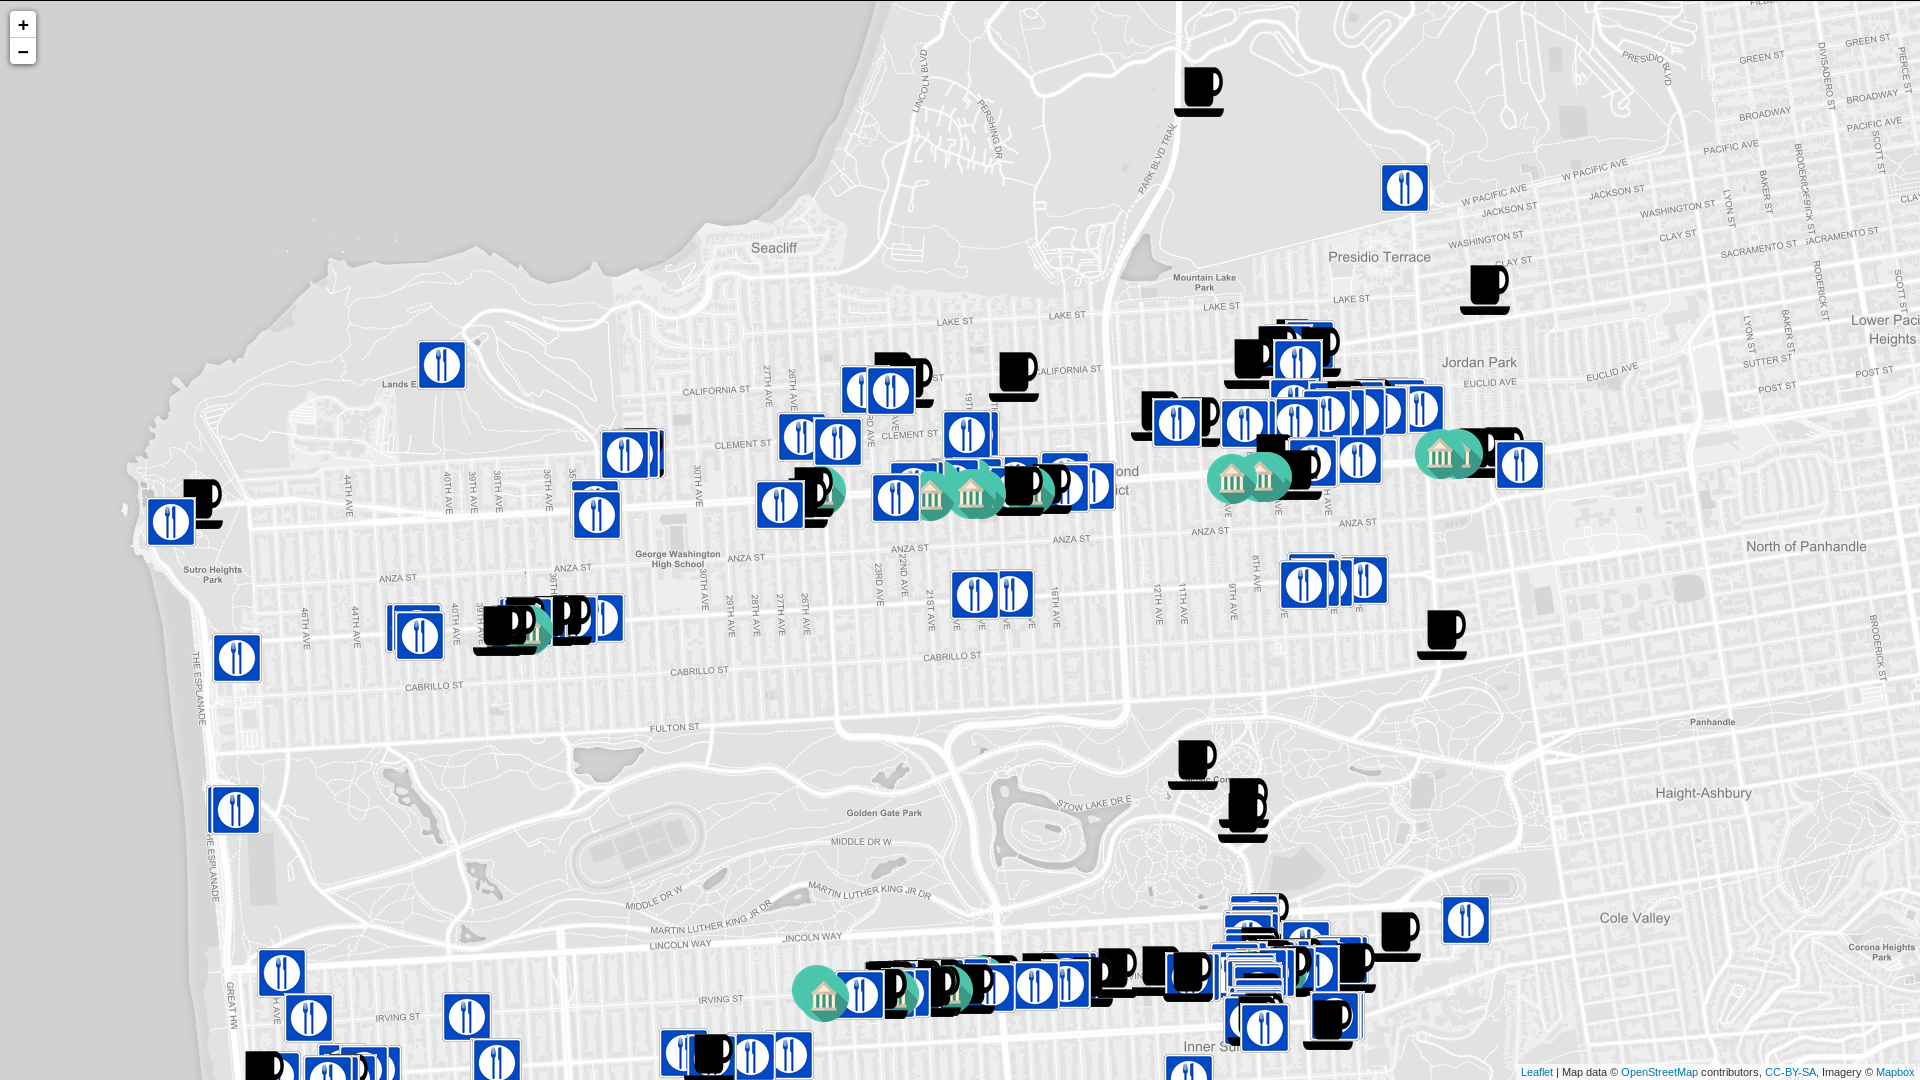
\includegraphics[width=0.8\textwidth]{graphics/cafes_restaurants_banks_larger.png}
		\caption{A map indicating public amenities (cafes, restaurants, banks) found at points of interest in OSM.}
		\label{fig:pois}
	\end{figure}
	
	Furthermore, we collect the vising duration of amenities. This information is offered by Google Places and FourSquare. The latter data is available via an API, however the access not free. We collected data from Google Places corresponding to the parking data's location. An example of the service is withing Google Maps for mobile phones. It displays typical \textit{visiting duration} or \textit{time spent} values and popularity of the place for specific points in time. The average values are based on the users' smart phone GPS sensors (cf. \cref{fig:visit_duration}). To obtain the duration values, we manually extract information from Google Maps. The duration information is aggregated by Google using a crowdsourcing approach. 
	
	\begin{figure}[!ht]
		\centering
		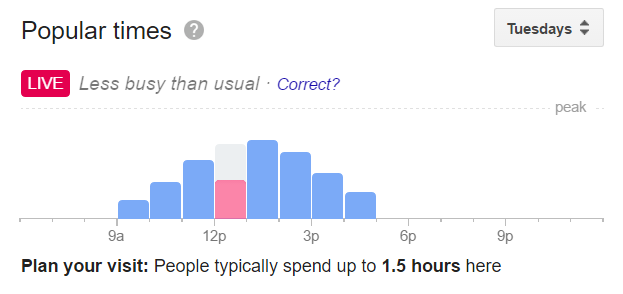
\includegraphics[width=0.8\textwidth]{graphics/google_visit_duration.png}
		\caption{An example of \textit{visiting duration} information found on Google Maps.}
		\label{fig:visit_duration}
	\end{figure}  
	
	In order to combine the parking and OSM data (or city data), both sets of data require a common location unit. The parking location units are provided together alongside the various types of parking data. The city data, on the other hand, references POI geometries, which are points expressed in a particular reference system, which differs from the one of the parking locations. Therefore, after establishing the coordinate systems of both geometries, we define a \textit{merge distance} that matches a parking space to a public amenity. 
	
	The merge distance can be intuitively understood as the radius around a public amenity. It is defined to represent the parking area that is relevant for a particular public amenity, or, more straightforward, the walking distance from the parked car to e.g., the restaurant, the office, the bank, etc. Concrete instances of the merging distance can be found in \cmmnt{\cref{experimental_setup:merging_parking_city_data}} the evaluation section.
	
\end{document}